\section{Messung} % (fold)
\label{sec:messung}
Im Folgenden Abschnitt werden die Messungen der Gitterkonstante von HOPG, sowie
der Plateauhöhen von Gold erläutert. Zum einlesen der Messdaten und für eine
einfache Rauschunterdrückung wird die freie Software \texttt{gwyddion}
\cite{gwyddion} benutzt. Für die Analyse der HOPG Struktur wird \texttt{python}
\cite{python3} verwendet.
Um die Plateauhöhen von Gold zu studieren wird die Software \texttt{WSxM} \cite{WSxM} genutzt.

Um mit dem Mikroskop verwertbare Bilder zu erzeugen, muss zunächst ein Stück
Platindraht mit einer Zange abgetrennt werden. Dabei ist es essentiell, den
Draht abzureissen, statt ihn abzuschneiden. Dadurch wird gewährleistet, dass
ein Ende des Drates eine sehr feine -- im Idealfall einatomige -- Spitze
aufweist.

Die Spitze wird in den Mikroskopschlitten eingelegt und die Probe mit Hilfe von
Piezzoelementen an diese herangefahren. Die Steuerung wird mit Hilfe der dem
Mikroskop beiliegenden Software durchgeführt.
Sobald der Abstand so klein ist, dass ein Tunnelstrom gemessen wird, fährt
die Probe ein zuvor definiertes Raster in $x$- und $y$-Richtung ab. Das so
entstehende Bild wird gespeichert und ausgewertet.

\subsection{Gittervektoren von HOPG}
\label{subsec:gitter}
Zunächst werden einige Testaufnahmen erstellt, um Mikroskopeinstellungen zu
finden, die die zu untersuchende Gitterstruktur erkennen lassen.
Der Bildausschnitt deckt dabei eine Fläche von $\num{2}\times\num{2}\,
\si{\nano\meter\squared}$ ab. Eine beispielhafte Aufnahme, nach Vorverarbeitung
durch \texttt{gwyddion}, ist in Abbildung \ref{fig:hopg1} dargestellt.
\begin{figure}
    \centering
    \includegraphics[width=0.5\linewidth]{build/plots/HOPG_downwards.pdf}
    \caption{Aufnahme von Graphit mit dem Rastertunnelmikroskop. Eine
             periodische Struktur ist klar zu erkennen.}
    \label{fig:hopg1}
\end{figure}
Offensichtlich taucht bei $x \approx \SI{1.05}{\nano\meter}$ eine Unstetigkeit
auf. Außerdem ist die Aufnahme im Bereich $y > \SI{1.5}{\nano\meter}$
anscheinend verzerrt. Diese Werte werden als grobe Selektion der Daten
benutzt, mit denen die Gittervektoren bestimmt werden.

In einem nächsten Schritt werden alle lokalen Maxima in einer Umgebung von
\num{12} Pixeln gesucht und markiert. Im zuvor gewählten Selektionsbereich
werden zudem zwei Korridore mit möglichst vielen Maxima gewählt, die sich an
der grob zu erkennenden Struktur der Gitterstruktur orientieren.
Die grobe Vorselektion, die Maxima und die Selektionskorridore sind in
Abbildung \ref{fig:hopg1_selektion} bis \ref{fig:hopg4_selektion} dargestellt.
An die Punkte innerhalb dieser Korridore werden in einem Least-Squares-Fit
lineare Funktionen angepasst und damit Richtungsvektoren bestimmt. Die Länge
dieser Vektoren wird duch Mittelung über alle benutzten Punkte bestimmt.
Dabei werden zwei Gittervektoren $\vec{a}_1$ und $\vec{a}_2$ bestimmt.
Die Vektoren sind in Abbildungen \ref{fig:hopg1_vektoren} bis
\ref{fig:hopg4_vektoren} eingezeichnet.
Zudem wird der Winkel zwischen beiden Vektoren bestimmt.
Diese Analyse wird für alle vier Messungen durchgeführt. Es ergeben sich die
in Tabelle \ref{tab:vektoren} aufgeführten Werte.
\begin{table}
    \centering
    \caption{
        Werte der durch Fit bestimmten Gittervektoren von HOPG. Es sind $x$-
        und $y$-Komponenten der Vektoren $\vec{a}_i$, deren Länge $a_i$, sowie
        der Winkel $\alpha$ zwischen beiden Vektoren aufgeführt.
    }
    \label{tab:vektoren}
    \begin{adjustbox}{center}
        \input{build/tex/table_vec.tex}
    \end{adjustbox}
\end{table}
Mittelung über alle Messungen ergibt
\begin{align*}
    \input{build/tex/avg_a1.tex}\,,\\
    \input{build/tex/avg_a2.tex}\,,\\
    \text{und}\qquad\input{build/tex/avg_a1_len.tex}\,,\\
    \input{build/tex/avg_a2_len.tex}\,,\\
    \text{sowie}\qquad\input{build/tex/avg_angle.tex}\,.
\end{align*}

Durch Vergleich mit den Literaturwerten \cite{STM-hopg} $\hat{a}
= \SI{2.461}{\angstrom}$ und dem erwarteten Winkel $\alpha = \SI{60}{\degree}$
lässt sich
eine Skalierung $s_x$ bzw. $s_y$ der $x$- und $y$- Achse finden, sodass die
gemessenen Werte für $\left|\vec{a}_i\right|$ mit diesen übereinstimmen.
Diese Transformation lässt sich mit einer Diagonalmatrix $S$ ausdrücken als
$\vec{a}_i \to S\vec{a}_i$ und die zu erfüllenden Bedingungen lauten
\begin{align*}
    \frac{S\vec{a}_1\vec{a}_2}
         {\sqrt{\left(S\vec{a}_1\right)^2 \left(S\vec{a}_2\right)^2}}
         &= \cos{\alpha}\,\\
         \text{und}\qquad\left(S\vec{a}_1\right)^2
         &= \left(S\vec{a}_1\right)^2 = \hat{a}^2\,.
\end{align*}
Daraus folgt für ein gegebenes $s_y$
\begin{align*}
    s_x^2 &= \frac{\hat{a}^2\cos{\alpha} - s_y^2 a_{1,y} a_{2,y}}
                  {a_{1,x} a_{2,x}}\,.
\end{align*}
Die Skalierungsfaktoren sind schließlich $\input{build/tex/scale_x.tex}$ und
$s_y = \num{1}$.
\clearpage
\begin{figure}
    \centering
    \subcaptionbox{
        Grobe Vorselektion der zum Fitten genutzten Datenpunkte.
        \label{fig:hopg1_selektion}
    }[0.6\linewidth]{\includegraphics[width=0.57\linewidth]{build/plots/hopg_down_selection.pdf}}
    \subcaptionbox{
        Gefittete Gittervektoren.
        \label{fig:hopg1_vektoren}
    }[0.39\linewidth]{\includegraphics[width=0.42\linewidth]{build/plots/hopg_down_arrows.pdf}}
    \caption{Vorselektion und Fitresultate der Bestimmung der Gittervektoren. HOPG Messung \num{1}.}
    \label{fig:hopg1_fit}
\end{figure}
\begin{figure}
    \centering
    \subcaptionbox{
        Grobe Vorselektion der zum Fitten genutzten Datenpunkte.
        \label{fig:hopg2_selektion}
    }[0.6\linewidth]{\includegraphics[width=0.57\linewidth]{build/plots/hopg_down-back_selection.pdf}}
    \subcaptionbox{
        Gefittete Gittervektoren.
        \label{fig:hopg2_vektoren}
    }[0.39\linewidth]{\includegraphics[width=0.42\linewidth]{build/plots/hopg_down-back_arrows.pdf}}
    \caption{Vorselektion und Fitresultate der Bestimmung der Gittervektoren. HOPG Messung \num{2}.}
    \label{fig:hopg2_fit}
\end{figure}
\begin{figure}
    \centering
    \subcaptionbox{
        Grobe Vorselektion der zum Fitten genutzten Datenpunkte.
        \label{fig:hopg3_selektion}
    }[0.65\linewidth]{\includegraphics[width=0.63\linewidth]{build/plots/hopg_up_selection.pdf}}
    \subcaptionbox{
        Gefittete Gittervektoren.
        \label{fig:hopg3_vektoren}
    }[0.34\linewidth]{\includegraphics[width=0.35\linewidth]{build/plots/hopg_up_arrows.pdf}}
    \caption{Vorselektion und Fitresultate der Bestimmung der Gittervektoren. HOPG Messung \num{3}.}
    \label{fig:hopg3_fit}
\end{figure}
\begin{figure}
    \centering
    \subcaptionbox{
        Grobe Vorselektion der zum Fitten genutzten Datenpunkte.
        \label{fig:hopg4_selektion}
    }[0.49\linewidth]{\includegraphics[width=0.49\linewidth]{build/plots/hopg_up-back_selection.pdf}}
    \subcaptionbox{
        Gefittete Gittervektoren.
        \label{fig:hopg4_vektoren}
    }[0.49\linewidth]{\includegraphics[width=0.49\linewidth]{build/plots/hopg_up-back_arrows.pdf}}
    \caption{Vorselektion und Fitresultate der Bestimmung der Gittervektoren. HOPG Messung \num{4}.}
    \label{fig:hopg4_fit}
\end{figure}
\clearpage

\subsection{Plateauhöhen einer Goldoberfläche}
\label{subsec:gold}
Im Folgenden werden mit Hilfe von \texttt{WSxM} die Höhendaten einer
Goldoberfläche ausgewertet. Entlang der in Abbildung \ref{fig:gold}
eingezeichneten Geraden ergeben diese Höhenwerte das in Abbildung
\ref{fig:gold-fit} dargestellte Höhenprofil.

An dieses Profil werden zwei Plateauhöhen $h_1$ und $h_2$ gefittet. Die
$x$-Werte werden dabei an den Stellen $x = \SI{60}{\nano\meter}$ und $x =
\SI{100}{\nano\meter}$ unterteilt.  Damit ergeben sie die Plateauhöhen für Gold
zu
\begin{equation*}
    \input{build/tex/plateau1.tex}\qquad\text{und}\qquad\input{build/tex/plateau2.tex}\,.
\end{equation*}
\begin{figure}
    \centering
    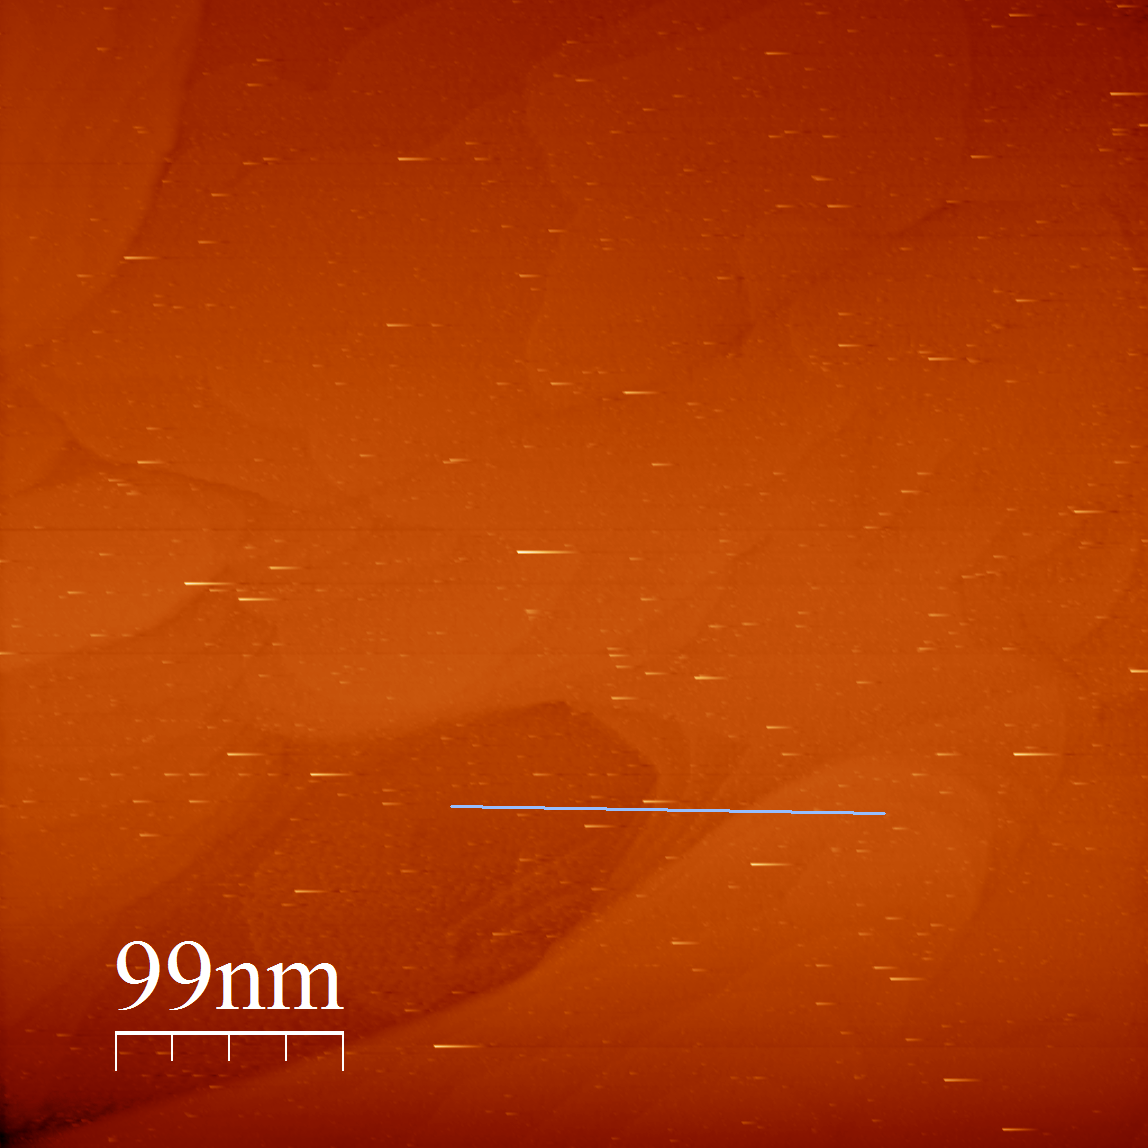
\includegraphics[width=0.9\linewidth]{raw/AU-1-View-2.png}
    \caption{
        Aufnahme einer Goldoberfläche. Entlang der eingezeichneten Linie
    wird ein Höhenprofil aufgenommen.
    }
    \label{fig:gold}
\end{figure}
\begin{figure}
    \centering
    \includegraphics[width=0.9\linewidth]{build/plots/au_plateaus.pdf}
    \caption{
        Höhenprofil einer Goldaufnahme mit Fit dreier Plateauhöhen zwischen $x
        = \SI{60}{\nano\meter}$ und $x = \SI{100}{\nano\meter}$.
    }
    \label{fig:gold-fit}
\end{figure}

\section{Diskussion}
\label{sec:diskussion}
Die Bestimmung der HOPG Gittervektoren verdeutlicht das hohe
Auflösungsvermögen der Rastertunnelmikroskopie. Selbst ohne Korrektur des
Koordinatensystems des Mikroskops sind die hier bestimmten Längen der Vektoren
vergleichbar mit den Literaturwerten $\hat{a} = \SI{2.461}{\angstrom}$. Die
Abweichung ist jedoch mit etwa $2\sigma$ signifikant. Der Winkel zwischen den
hier bestimmten Vektoren ist innerhalb der
Messfehler verträglich mit dem erwarteten Wert von \SI{60}{\degree}.

Das Höhenprofil von Gold liefert Werte für Plateauhöhen, die etwa dem doppelten
Literaturwert für den Gitterabstand \SI{407.82}{\pico\meter} von Gold
entsprechen. Diese Abweichung kann nur teilweise auf den Einfluss von
Hystereseeffekten der Piezzo-Kristalle zurückgeführt werden, da diese, wie in
\ref{ssub:piezokristalle} beschrieben, gering sein sollten.
%%% das hier ist anscheinend quatsch. Erst ein effekt nach mehreren Tagen
% Möglicherweise stellt die Abnutzung der Mikroskopspitze einen bedeutenden
% systematischen Fehler dar, was weiter untersucht werden müsste.
Die
Plateaukanten könnte mehr als einer Atomschicht entsprechen, was ein
ganzzahliges Vielfaches der Gitterkonstante als Kantenhöhe erwarten ließe.
Zudem ist nicht ohne weiteres klar, welche Netzebene in dem Bild betrachtet
wird.
Unter dieser Annahme wäre das hier gemessene Ergebnis mit mit einer Shichtdicke
von \num{2} Atomen kompatibel. Jedoch müsste auch die Gültigkeit dieser Annahme
weiter untersucht werden.
